\documentclass{beamer}
\usepackage[utf8]{inputenc}
\usepackage{url}
\usepackage{hyperref}
\graphicspath{{./fig/aula4}}

% Configurando layout para mostrar codigos C++
\usepackage{listings}
\lstset{
  language=HTML,
  basicstyle=\ttfamily\small, 
  keywordstyle=\color{blue}, 
  stringstyle=\color{red}, 
  commentstyle=\color{red}, 
  extendedchars=true, 
  showspaces=false, 
  showstringspaces=false, 
  numbers=left,
  numberstyle=\tiny,
  breaklines=true, 
  backgroundcolor=\color{green!10},
  breakautoindent=true, 
  captionpos=b,
  xleftmargin=0pt,
}

\date{}
\title{Desenvolvimento Web Básico}
\subtitle{Aula 4}

\usetheme{lucid}

\begin{document}
\frame{
 \titlepage
}

%--------------------------------------------------------------------------
\begin{frame}{Na aula de hoje...} 
\tableofcontents 
\end{frame}

%-----------------------------------------------------
\section{Bordas}
\begin{frame}{Bordas CSS}
	Propriedades de borda
 \begin{itemize}
  \item \textbf{dotted} - Define uma borda pontilhada
	\item \textbf{dashed} - Define uma borda tracejada
	\item \textbf{solid} - Define uma borda sólido
	\item \textbf{double} - Define uma margem dupla
  \item \textbf{groove} - Define uma borda sulcada 3D. O efeito depende do valor border-color
 \end{itemize}

\end{frame}
%-----------------------------------------------------
\begin{frame}{Bordas CSS}
	Propriedades de borda
 \begin{itemize}
	\item \textbf{ridge} - Define uma borda ridged 3D. O efeito depende do valor border-color
	\item \textbf{inset} - Define uma borda inset 3D. O efeito depende do valor border-color
	\item \textbf{outset} - Define uma borda início 3D. O efeito depende do valor border-color
	\item \textbf{none} - Define sem fronteira
	\item \textbf{hidden} - Define uma borda escondida
 \end{itemize}
\end{frame}
%-----------------------------------------------------
\begin{frame}{Bordas CSS}
Para editar partes da borda:
\begin{itemize}
	\item \textbf{border-top-style:} dotted;
  \item \textbf{border-right-style:} solid;
  \item \textbf{border-bottom-style:} dotted;
  \item \textbf{border-left-style:} solid;
  \item \textbf{border-width:} 20px;
 \end{itemize}
 \tiny Fontes: \cite{wschool2018html, purewal2014learning}
\end{frame}
%-----------------------------------------------------
\section{Estilo com base em estado}
\begin{frame}{CSS com base no estado}
É possível estilizar elementos com base no estado deles:\\
O CSS abaixo estiliza um link de verde quando não visitado, rosa quando visitado e sem decoração ao passar do mouse.
\begin{center}
		  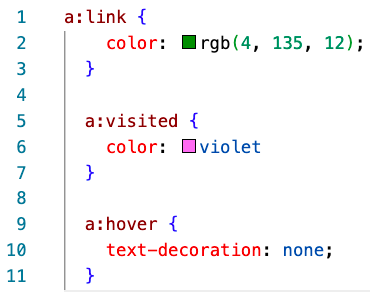
\includegraphics[height=0.4\paperheight]{fig/aula2/css_estado.png} \\
	  \end{center}
 \tiny Fontes: \cite{mdn2023}
\end{frame}

%-----------------------------------------------------
\section{Função CSS}
\begin{frame}{CSS Função}
Uma função consiste em chamar o nome de uma uma função e um par de perenteses, entre os parenteses são iformados os parâmetros.\\
No caso da função \textbf{calc()} o desenvolvedor inform que a largura da div deve ser 90\% do bloco onde ela está, menos 30px.\\
\begin{columns}
\begin{column}{0.5\textwidth}
        \begin{center}
		  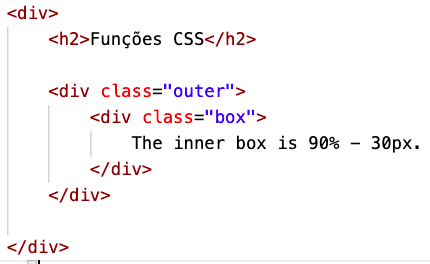
\includegraphics[height=0.4\paperheight]{fig/aula2/layout_html1.png} \\
		  \tiny{Código HTML}
	  \end{center}
   \end{column}
   \begin{column}{0.5\textwidth}
        \begin{center}
		  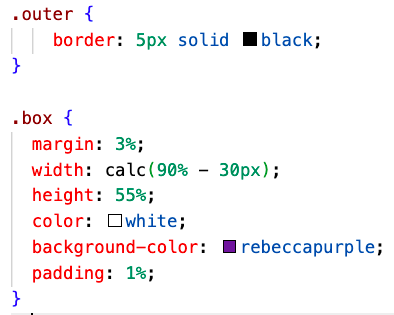
\includegraphics[height=0.4\paperheight]{fig/aula2/layout_css2.png} \\
		  \tiny{Código CSS}
	  \end{center}
	  
   \end{column}
\end{columns}
 \tiny Fontes: \cite{mdn2023}
\end{frame}
%-----------------------------------------------------
\begin{frame}{CSS Função}
Outro exemplo de função é a rotate aplicada a propriedade transform.\\
\begin{columns}
\begin{column}{0.5\textwidth}
        \begin{center}
		  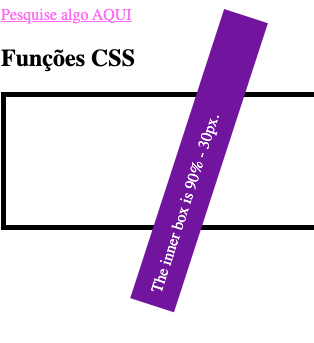
\includegraphics[height=0.4\paperheight]{fig/aula2/layout_html2.png} \\
		  \tiny{Saída do Código HTML}
	  \end{center}
   \end{column}
   \begin{column}{0.5\textwidth}
        \begin{center}
		  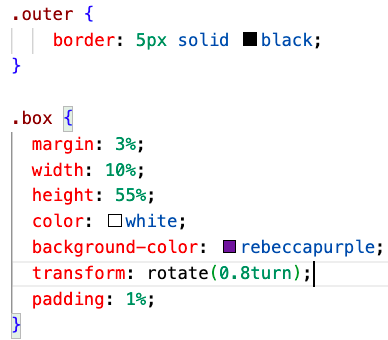
\includegraphics[height=0.4\paperheight]{fig/aula2/layout_css1.png} \\
		  \tiny{Código CSS: Edite o código anterior para width: 20\% e acrescente a propriedade transform.}
	  \end{center}
	  
   \end{column}
\end{columns}
 \tiny Fontes: \cite{mdn2023}
\end{frame}

%-----------------------------------------------------
\section{CSS Regras}
\begin{frame}{CSS Regras}
Regras CSS são aplicadas com o operador \@. E descrevem formatações CSS que só serão aplicadas dependendo de uma determinada condição.
\begin{columns}
\begin{column}{0.5\textwidth}
        A regra ao lado será aplicada apenas se o monitor que exibe o seu site tiver mais de 30em
   \end{column}
   \begin{column}{0.5\textwidth}
        \begin{center}
		  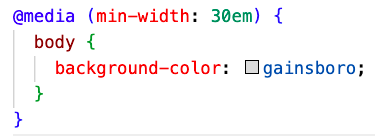
\includegraphics[height=0.2\paperheight]{fig/aula2/layout_css3.png} \\
		  \tiny{Código CSS: Acrescente este código ao CSS anterior.}
	  \end{center}
	  
   \end{column}
\end{columns}
Teste a visualização no modo celular nas opções de "inspecionar" do Chrome.\\
 \tiny Fontes: \cite{mdn2023}
\end{frame}

%-----------------------------------------------------
\section{Atividades}
\begin{frame}{Atividade 1}
Sobre barras de navegação. Vamos utilizar alguns conceitos conhecidos para criar uma barra de navegação 
vertical.
	\begin{center}
		  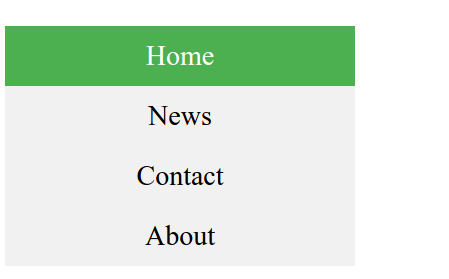
\includegraphics[height=0.4\paperheight]{fig/aula2/aep_1_2.png} \\
	  \end{center}
\end{frame}
%-----------------------------------------------------
\begin{frame}{Atividade 2}
Reproduza a página a seguir utilizando propriedades de borda;
  \begin{center}
    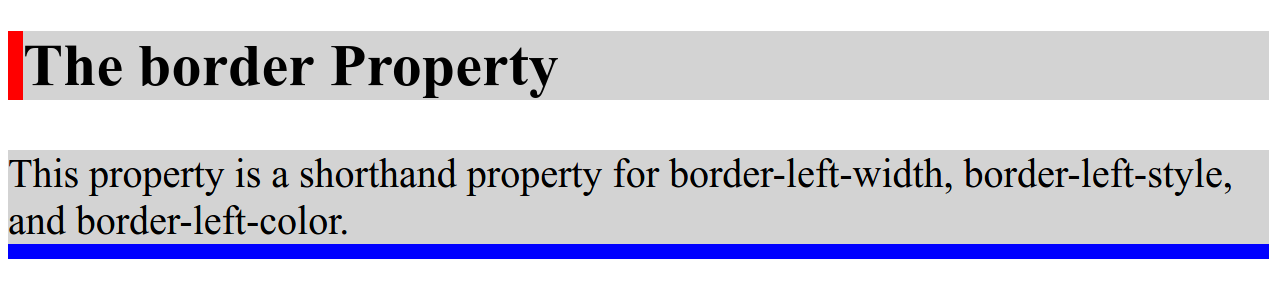
\includegraphics[height=0.2\paperheight]{fig/aula2/AEP_1_1.png} \\
  \end{center}
\end{frame}

%-----------------------------------------------------



%----------------------------------------------------------------------------
\section{Referências}

\begin{frame}{Referências}%[allowframebreaks]
\small
\begin{center}
\tiny
\bibliographystyle{apalike}
\bibliography{ref_aula}
\end{center}
\end{frame}

\end{document}

\end{document}